%\documentclass[main.tex]{subfiles}
\documentclass[a4paper, landscape]{article}


\usepackage{tikz}
\usetikzlibrary{positioning,shapes}
%\usepackage[a4paper,margin=1in,landscape]{geometry}

\newcommand{\red}{red!50}
\newcommand{\green}{green!50}
\newcommand{\blue}{blue!50}

\tikzset{
    line/.style = { line width=2pt, },
    arrow/.style = { ->,line width=1pt, },
    invisible/.style = { inner sep=0, minimum size=0, },
    write/.style = { text=black,font=\LARGE,inner sep=0, },
    wee/.style = { text=black,font=\Large,inner sep=0, },
    blob/.style = { write,minimum width=2cm, },
}

\newcommand{\hadron}[5]{
    \coordinate (a) at (-6,#2*3);

    \draw [line] (c) -- +(-6,#2*2) -- +(-12,#2*2);
    \draw [line] (-12,#2*3) -- (a) -- (0,#2*5);
    \draw [line] (-12,#2*4) -- (-6,#2*4) -- (0,#2*6);

    \draw [arrow] (-3.5,#2*1.75) -- node [#4,wee,yshift=#2*2mm] {$x_#3P_#3$} +(1.5,-#2*0.5);
    \draw [arrow] (-10.5,#2*4.5) -- node [#4,wee,yshift=#2*2mm] {$P_#3$} +(2,0);

    \node [ellipse,fill=\red,minimum height=4cm,blob] at (a) {$f_#5(x_#3, \mu_F)$};

    \node [write] at (-12.75,#2*3) {$h_#3$};
}

\newcommand{\ssplit}[7]{
    \node [invisible, above right={#2*cos(#5)} and {#2*sin(#5)} of #1] (#6) {};
    \node [invisible, above right={#3*cos(#4+#5)} and {#3*sin(#4+#5)} of #1] (#7) {};
    \draw [line] (#1) -- (#6);
    \draw [line] (#1) -- (#7);
}
\pagenumbering{gobble}

\begin{document}
\hspace{-8cm}
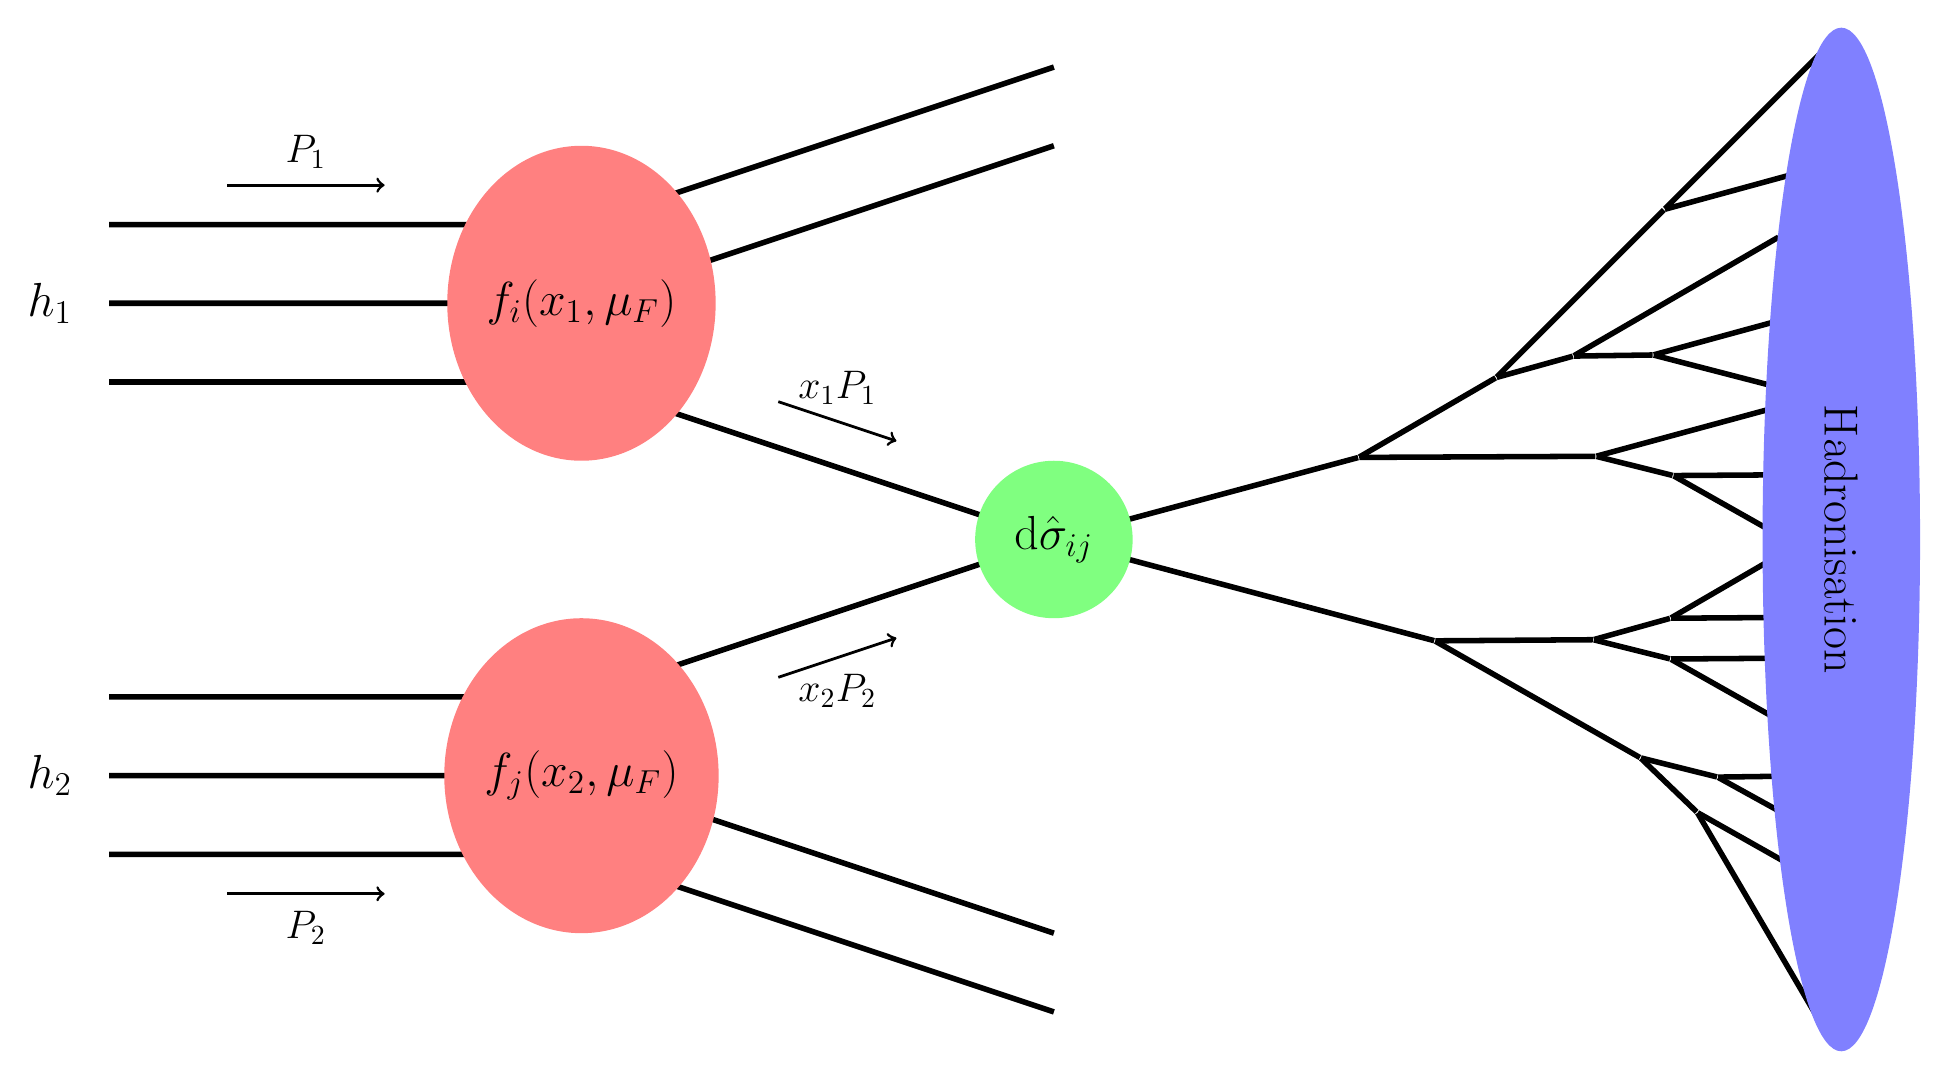
\begin{tikzpicture}

    \coordinate (c) at (0,0);

    \hadron{c}{1}{1}{above}{i}
    \hadron{c}{-1}{2}{below}{j}

    \ssplit{c}{4}{5}{30}{75}{a1}{a2}

    \ssplit{a1}{2}{3}{30}{60}{b1}{b2}
    \ssplit{b1}{3}{1}{30}{45}{c1}{c2}
    \ssplit{c2}{3}{1}{30}{60}{d1}{d2}
    \ssplit{b2}{3}{1}{30}{75}{e1}{e2}
    \ssplit{c1}{3}{2}{30}{45}{f1}{f2}
    \ssplit{d2}{2}{2}{30}{75}{m1}{m2}
    \ssplit{e2}{2}{2}{30}{90}{n1}{n2}

    \ssplit{a2}{2}{3}{30}{90}{g1}{g2}
    \ssplit{g1}{1}{1}{30}{75}{h1}{h2}
    \ssplit{g2}{1}{1}{30}{105}{j1}{j2}
    \ssplit{h1}{2}{2}{30}{60}{k1}{k2}
    \ssplit{j1}{1}{1}{30}{90}{i1}{i2}
    \ssplit{j2}{2}{3}{30}{120}{l1}{l2}
    \ssplit{h2}{2}{2}{30}{90}{o1}{o2}

    \node [circle,fill=\green,blob] at (c) {$\mathrm{d}\hat\sigma_{ij}$};

    \coordinate (h) at (10,0);
    \fill [\blue] (h) ellipse (1 and 6.5);
    \node [rotate=270,blob] at (h) {Hadronisation};

\end{tikzpicture}




%\begin{figure}
%    \centering
%    \begin{subfigure}[b]{0.3\textwidth}
%        \hspace*{1em}\raisebox{1.1cm}{ % needed to align the diagrams
%        \begin{tikzpicture}
%        	\begin{feynman}[small]
%        		\vertex (v1);
%          
%        		\vertex[above left = 0.8cm of v1, yshift=-0.2cm] (i1);
%        		\vertex[below left =  0.8cm of v1, yshift=+0.2cm] (i2);
%        		\vertex[right = of v1] (v2);			
%        		\vertex[right = of v2] (v3);			
%        		
%        		\vertex[above right = 0.8cm of v3, yshift=-0.2cm] (f1);
%        		\vertex[right = 0.70cm of v3] (f2);
%        		\vertex[below right = 0.8cm of v3, yshift=+0.2cm] (f3);
%
%        		\diagram*{
%        			(i1) -- (v1) -- [out=60, in=120] (v2) -- [out=60, in=120] (v3) -- (f1),
%        			(i2) -- (v1) -- [out=-60, in=-120] (v2) -- [out=-60, in=-120] (v3) -- (f3),
%                    (v3) -- (f2),
%                
%        		};
%        	\end{feynman}
%        \end{tikzpicture}}
%    \caption{} \label{fig:topologya}
%    \end{subfigure}
%    \begin{subfigure}[b]{0.3\textwidth}
%        \hspace*{1em}
%        \begin{tikzpicture}
%    	\begin{feynman}[small]
%    		\vertex (v1);
%      
%    		\vertex[above left = 0.8cm of v1, yshift=-0.2cm] (i1);
%    		\vertex[below left =  0.8cm of v1, yshift=+0.2cm] (i2);
%    		\vertex[above right = of v1] (v2);			
%    		\vertex[below right = of v1] (v3);			
%    		\vertex[right = of v2] (v4);			
%    		\vertex[right = of v3] (v5);			
%    		
%    		\vertex[above right = 0.8cm of v4] (f1);
%    		\vertex[below right = 0.5cm of v5, yshift=-0.4cm] (f2);
%    		\vertex[below right = 0.5cm of v5, xshift=+0.4cm] (f3);
%    		
%    		\diagram*{
%    			(i1) -- (v1) -- (v2) -- (v4) -- (f1),
%    			(i2) -- (v1) -- (v3) -- (v5) -- (f2),
%                (v2) -- (v3),
%                (v4) -- (v5),
%                (v5) -- (f3),
%    		};
%    	\end{feynman}
%    \end{tikzpicture}
%    \caption{} \label{fig:topologyb}
%    \end{subfigure}
%    \begin{subfigure}[b]{0.3\textwidth}
%        \hspace*{1em}
%        \begin{tikzpicture}
%    	\begin{feynman}[small]
%    		\vertex (i1);
%    		\vertex[below right= 0.8cm of i1] (v1);
%    		\vertex[right = of v1] (v2);
%    		\vertex[yshift=0.3cm, right = 0.8cm of v2] (v3);
%    		\vertex[above right = 0.8cm of v3] (f1);			
%    		
%    		\vertex[below = of v1] (v7) ;
%    		\vertex[below left = 0.8cm of v7] (i2) ;
%    		\vertex[right = of v7] (v6) ;
%    		\vertex[yshift=-0.3cm, right = 0.8cm of v6] (v5) ;
%    		\vertex[below right = 0.8cm of v5] (f3) ;
%    		
%    		\vertex[xshift=0.6cm, yshift=0.2cm, below = of v3] (v4);
%    		\vertex[right = 0.8cm of v4] (f2) ;		
%    		
%    		\diagram*{
%    			(i1) -- (v1) -- (v2) -- (v3),
%    			(i2) -- (v7) -- (v6) -- (v5),
%    			(v3) -- (f1),
%    			(v3) -- (v4) -- (v5),
%    			(v4) -- (f2),
%    			(v5) -- (f3),
%    			(v1) -- (v7),
%    			(v2) -- (v6),
%    		};
%    	\end{feynman}
%    \end{tikzpicture}
%    \caption{} \label{fig:topologyc}
%    \end{subfigure}
%\caption{Examples of diagram topologies associated with five-particle Feynman diagrams. It is easy to see that topologies (a) and (b) can be obtained from topology (c) by pinching some of its propagators.}
%\label{fig:topologies}
%\end{figure}

%\begin{figure}
%    \centering
%    \begin{tikzpicture}
%
%        %axes
%        \draw[thick,->] (-3.5,0) -- (3.5,0) node[anchor=north west] {$\nu_1$};
%        \draw[thick,->] (0,-3.5) -- (0,3.5) node[anchor=south east] {$\nu_2$};
%
%        %dots and axes labels
%        \draw[fill] (0,0) circle (1pt) node[anchor=north east] {$0$};
%        \foreach \i in {-3,-2,-1,1,2,3}
%            {
%            \draw[fill] (0,\i ) circle (1pt) node[anchor=east] {$\i$};
%            \draw[fill] (\i,0) circle (1pt) node[anchor=north] {$\i$};
%            \foreach \j in {-3,-2,-1,1,2,3}
%                \draw[fill] (\j, \i) circle (1pt);
%            }
%
%        %lines separating sectors
%        \draw[thick, blue] (0.5, -3.5) -- (0.5, 3.5);
%        \draw[thick, blue] (-3.5, 0.5) -- (3.5, 0.5);
%
%        \node at (2, 2.5) {$\bm{\theta_I} = \{1, 1\}$};
%        \node at (-2, 2.5) {$\bm{\theta_{II}} = \{0, 1\}$};
%        \node at (2, -2.5) {$\bm{\theta_{III}} = \{1, 0\}$};
%        \node at (-2, -2.5) {$\bm{\theta_{IV}} = \{0, 0\}$};
%
%
%        \clip (-3.3,-3.3) rectangle (0.3, 0.3);
%        \foreach \i in {-12,...,0}
%            \draw[dashed, red, samples=100] plot function{-x+(0.3+0.5*\i)} node[right] {};
%    \end{tikzpicture}
%    \caption{Caption}
%    \label{fig:sectors}
%\end{figure}


%\begin{figure}
%    \centering
%    \begin{subfigure}[b]{0.4\textwidth}
%    \begin{tikzpicture}
%        %axes
%        \draw[thick,->] (-3.5,0) -- (3.5,0) node[anchor=north west] {$\nu_1$};
%        \draw[thick,->] (0,-3.5) -- (0,3.5) node[anchor=south east] {$\nu_2$};
%        %dots and axes labels
%        \draw[fill] (0,0) circle (1pt) node[anchor=north east] {$0$};
%        \foreach \i in {-3,-2,-1,1,2,3}
%            {
%            \draw[fill] (0,\i ) circle (1pt) node[anchor=east] {$\i$};
%            \draw[fill] (\i,0) circle (1pt) node[anchor=north] {$\i$};
%            \foreach \j in {-3,-2,-1,1,2,3}
%                \draw[fill] (\j, \i) circle (1pt);
%            }
%        %lines separating sectors
%        \draw[thick, blue] (0.5, -3.5) -- (0.5, 3.5);
%        \draw[thick, blue] (-3.5, 0.5) -- (3.5, 0.5);
%
%        \node at (2, 2.5) {$\bm{\theta_I} = \{1, 1\}$};
%        \node at (-2, 2.5) {$\bm{\theta_{II}} = \{0, 1\}$};
%        \node at (2, -2.5) {$\bm{\theta_{III}} = \{1, 0\}$};
%        \node at (-2, -2.5) {$\bm{\theta_{IV}} = \{0, 0\}$};
%
%        \clip (-3.3,-3.3) rectangle (0.3, 0.3);
%        \foreach \i in {-12,...,0}
%            \draw[dashed, red, samples=100] plot function{-x+(0.3+0.5*\i)} node[right] {};
%    \end{tikzpicture}
%    \caption{Each point $(\nu_1, \nu_2)$ in the $\mathbb{Z}^2$ lattice corresponds to the $d$-dimensional Feynman integral $I(\nu_1, \nu_2)$. The lattice is divided into sectors as defined through Eq.~\ref{eq:sectors}. They are ordered $\bm{\theta}_{I}>\bm{\theta}_{II},\,\bm{\theta}_{III}>\bm{\theta}_{IV}$. In particular, sector $\bm{\theta}_{IV}$ is trivially 0.} 
%    \label{fig:IBPsectors}
%    \end{subfigure}
%    \hfill
%    \hspace*{1em}\raisebox{0.9cm}{ % needed to align the diagrams
%    \begin{subfigure}[b]{0.45\textwidth}
%    \begin{tikzpicture}
%      %axes
%        \draw[thick,->] (-0.5,0) -- (5.5,0) node[anchor=north west] {$\nu_1$};
%        \draw[thick,->] (0,-0.5) -- (0,6.5) node[anchor=south east] {$\nu_2$};
%
%        %dots and axes labels
%        \draw[fill] (0,0) circle (1pt) node[anchor=north east] {$0$};
%        \foreach \i in {1,...,6}
%            {
%            \draw[fill] (0,\i ) circle (1pt) node[anchor=east] {$\i$};
%            \draw[fill] (\i,0) circle (1pt) node[anchor=north] {$\i$};
%            \foreach \j in {1,...,5}
%                \draw[fill] (\j, \i) circle (1pt);
%            }
%
%        %lines separating sectors
%        \draw[thick, blue] (0.5, -0.5) -- (0.5, 6.5);
%        \draw[thick, blue] (-0.5, 0.5) -- (5.5, 0.5);
%
%        \draw[orange, thick, ->] (5, 4) edge (5,3) (5, 3) edge (4,3) (4,3) edge (4,2) (4,2) edge (3,2) (3,2) edge (2,2) (2,2) edge (2,1) (2, 1) -- (1,1);
%        
%        \node at (5, 6.5) {$\bm{\theta_I}$};
%        \node at (1, 1) [anchor=south] {$\text{MI}(1, 1)$};
%        \node at (5, 4) [anchor=south] {$I(5, 4)$};
%    \end{tikzpicture}
%    \caption{A hypothetical reduction pathway within the top sector $\bm{\theta}_I$. An integral $I(5, 4)$ is reduced to the master integral $\text{MI}(1,1)$ through a series of IBP relations lowering the denominator exponents.} \label{fig:IBPreduction}
%    \end{subfigure}
%    }
%    \caption{A visualisation of integrals and sectors used in the IBP reduction as a lattice of points ($N=2$).}
%    \label{fig:IBPschematic}
%\end{figure}

%\begin{figure}
%    \centering
%        \begin{tikzpicture}
%        	\begin{feynman}
%        		\vertex (v1);
%          
%        		\vertex[right = of v1] (v2);			
%        		\vertex[below = of v2] (v3);			
%        		\vertex[left = of v3] (v4);			
%          
%        		\vertex[above left = 0.7cm of v1] (i1) {$p_1$};
%        		\vertex[above right =  0.7cm of v2] (i2) {$p_2$};
%        		\vertex[below right =  0.7cm of v3] (i3) {$p_3$};
%        		\vertex[below left =  0.7cm of v4] (i4) {$p_4$};
%
%                \node (dot) at ($(v2)!0.5!(v3)$);
%                \draw[fill] (dot) circle (2pt);
%          
%        		\diagram*{
%                    (v1) -- (v2) -- (v3) -- (v4) -- [momentum=$k_1$] (v1),
%                    (i1) -- (v1),
%                    (i2) -- (v2),
%                    (i3) -- (v3),
%                    (i4) -- (v4),
%                    };
%        	\end{feynman}
%        \end{tikzpicture}
%    \caption{One-loop box Feynman diagram $I_\text{box}(1,1,2,1)$ with a `dotted' propagator. The corresponding denominators are: $\{k_1^2, (k_1-p_1)^2, \left((k_1-p_1-p_2)^2\right)^2, (k_1+p_4)^2\}$\,.} \label{fig:1Lboxdot}
%\end{figure}

%\begin{figure}
%    \centering
%    \begin{adjustbox}{minipage=\textwidth,scale=0.9}
%    \raisebox{0.2cm}{
%    \begin{subfigure}[b]{0.25\linewidth}
%        \hspace*{1em}
%        \begin{tikzpicture}
%    	\begin{feynman}[small]
%    		\vertex (v1);
%    		\vertex[above left = 0.8cm of v1] (i1) {$p_5$};
%    		\vertex[right = of v1] (v2);
%    		\vertex[yshift=0.3cm, right = 0.8cm of v2] (v3);
%    		\vertex[above right = 0.8cm of v3] (f1) {$p_1$};			
%    		
%    		\vertex[below = of v1] (v7) ;
%    		\vertex[below left = 0.8cm of v7] (i2) {$p_4$};
%    		\vertex[right = of v7] (v6) ;
%    		\vertex[yshift=-0.3cm, right = 0.8cm of v6] (v5) ;
%    		\vertex[below right = 0.8cm of v5] (f3) {$p_3$};
%    		
%    		\vertex[xshift=0.6cm, yshift=0.2cm, below = of v3] (v4);
%    		\vertex[right = 0.8cm of v4] (f2) {$p_2$};		
%
%            \draw ($(v7)!0.5!(v6)$) node[cross,red] (5cm) {};
%            \draw ($(v4)!0.5!(v5)$) node[cross,red,rotate=45] (5cm) {};
%            
%    		\diagram*{
%    			(i1) -- (v1) -- (v2) -- (v3),
%    			(i2) -- (v7) -- (v6) -- (v5),
%    			(v3) -- (f1),
%    			(v3) -- (v4) -- (v5),
%    			(v4) -- (f2),
%    			(v5) -- (f3),
%    			(v1) -- (v7),
%    			(v2) -- (v6),
%    		};
%    	\end{feynman}
%    \end{tikzpicture}
%    \caption{} \label{fig:topologyc}
%    \end{subfigure}
%    }
%    %\end{adjustbox}
%    \hspace{1.3cm}
%    %\begin{adjustbox}{minipage=\linewidth,scale=0.4}
%    \begin{subfigure}[b]{0.25\linewidth}
%        \hspace*{1em}
%        \begin{tikzpicture}
%        \begin{feynman}[small]
%			\vertex (v1);
%			\vertex[left = 0.8cm of v1] (i1) {$p_5$};
%			\vertex[above right =1cm of v1] (v2);
%			\vertex[below right =1cm of v1] (v3);				
%			\vertex[yshift=0.3cm, right = 0.7cm of v2] (v4);	
%			\vertex[yshift=-0.6cm, right = 0.7cm of v4] (v5);
%			\vertex[yshift=-0.3cm, right = 0.7cm of v3] (v7);
%			\vertex[yshift=0.6cm, right = 0.7cm of v7] (v6);	
%			\vertex[above right = 0.8cm of v4] (i2) {$p_1$};
%			\vertex[yshift=0.2cm, right = 0.8cm of v5] (i3) {$p_2$};
%			\vertex[yshift=-0.2cm, right = 0.8cm of v6] (i4) {$p_3$};
%			\vertex[below right = 0.8cm of v7] (i5) {$p_4$};
%			
%            \draw ($(v7)!0.5!(v3)$) node[cross,red,rotate=60] (5cm) {};
%            \draw ($(v6)!0.5!(v5)$) node[cross,red] (5cm) {};
%            
%			\diagram*{
%				(i1) -- (v1) -- (v2) -- (v3) -- (v1),
%				(v2) -- (v4) -- (v5) -- (v6) -- (v7) -- (v3),
%				(v4) -- (i2),
%				(v5) -- (i3),
%				(v6) -- (i4),
%				(v7) -- (i5),
%			};
%		\end{feynman}
%        \end{tikzpicture}
%    \caption{} \label{fig:topologyc}
%    \end{subfigure}
%    %\end{adjustbox}
%    \hspace{1.3cm}
%    %\begin{adjustbox}{minipage=\linewidth,scale=0.4}
%    \raisebox{0.2cm}{
%    \begin{subfigure}[b]{0.25\linewidth}
%        \hspace*{1em}
%        \begin{tikzpicture}
%    	\begin{feynman}[small]
%    		\vertex (v1);
%      
%    		\vertex[left = 0.8cm of v1] (i1) {$p_5$};
%    		\vertex[above right = of v1] (v2);			
%    		\vertex[below right = of v1] (v3);			
%    		\vertex[right = of v2] (v4);			
%    		\vertex[right = of v3] (v5);			
%    		
%    		\vertex[above right = 0.8cm of v4] (i2) {$p_1$};
%    		\vertex[below right = 0.7cm of v5, yshift=-0.2cm] (i3) {$p_3$};
%    		\vertex[below right = 0.5cm of v5, xshift=+0.4cm] (i4) {$p_2$};
%    		\vertex[below =  0.7cm of v3] (i5) {$p_4$};
%    		
%    		\diagram*{
%                (i1) -- (v1) -- (v2) -- (v4) -- (i2),
%                (v1) -- (v3) -- (v5) -- (i3),
%                (v2) -- (v3),
%                (v4) -- (v5),
%                (v5) -- (i4),
%                (v3) -- (i5),
%    		};
%    	\end{feynman}
%    \end{tikzpicture}
%    \caption{} \label{fig:topologyb}
%    \end{subfigure}
%    }
%    \end{adjustbox}
%\caption{A simple example of possible non-IBP relations between integrals within different (maximal) topologies. Integrals in lower sectors often map to each other. The red crosses denote a vanishing denominator, i.e. the corresponding $\nu_i$ is 0. Here, diagrams $(a)$ and $(b)$ both collapse onto diagram $(c)$. Such relations are often hard to discover just from analysing the propagators of the integrals, especially if the two families use vastly different conventions for loop momentum routing. However, a visual representation often makes spotting these relations trivial.}
%\label{fig:topologies}
%\end{figure}


%\begin{table}[b]
%	\begin{center}
%		\begin{tabular}{|c|c|c|c|}
%            \hline
%            External masses & Type & Topology & Publications \\
%			\hline
%            \multirow{2}{0cm}{0} & planar & penta-box & \cite{Gehrmann:2015bfy,Papadopoulos:2015jft, Gehrmann:2018yef, Abreu:2018aqd, Chicherin:2020oor} \\
%            \cline{2-4}
%            & \multirow{2}{2cm}{non-planar} & hexa-box & \cite{Chicherin:2018mue, Chicherin:2017dob, Chicherin:2018ubl, Chicherin:2018wes, Abreu:2018rcw, Chicherin:2020oor, Abreu:2018aqd} \\
%            & & double-pentagon & \cite{Chicherin:2018old, Abreu:2018aqd, Chicherin:2020oor} \\
%            \hline
%            \multirow{2}{0cm}{1} & planar & penta-box & \cite{Abreu:2020jxa, Chicherin:2021dyp, Canko:2020ylt} \\
%            \cline{2-4}
%            & \multirow{2}{2cm}{non-planar} & hexa-box & \cite{abreu2021twoloop, Kardos:2022tpo, Papadopoulos:2019iam, Chicherin:2021dyp} \\
%            & & double-pentagon & N/A \\
%            \hline
%		\end{tabular}
%\end{center}
%\caption{Selected works relevant to the computation of two-loop, five-point master integral bases. At the time of writing, results for the one-mass non-planar double-pentagon family are not available in literature.}
%\label{tab:MIs}
%\end{table}

%	\begin{tikzpicture}[scale=0.4]
%        \begin{feynman}
%		\filldraw[gray!50,draw=black] (0,0) ellipse (4 and 2);
%		\draw[fill=white,draw=black,] (-2.5,0) ellipse (0.7cm and 1cm) node {\small $k_1$};
%		\draw[fill=white,draw=black,] (-.9,0) ellipse (0.7cm and 1cm) node {\small $k_2$};
%		\draw[fill=white,draw=black,] (+2.5,0) ellipse (0.7cm and 1cm) node {\small $k_L$};
%        \node (ldots) at (0.8, 0) {$\ldots$};
%
%        \node (kL) at (2.5, 0);
%        \ddd{kL.center}{2cm}{d1}{d2}{d3}{0}{20};
%		
%        \draw[thick] (3, 1.32) -- (5,3) node [anchor=south west] {$p_3$};
%		\draw[thick] (3, -1.32) -- (5,-3) node [anchor=north west] {$p_n$};
%		\draw[thick] (-3, 1.32) -- (-5,3) node [anchor=south east] {$p_2$};
%		\draw[thick] (-3, -1.32) -- (-5,-3) node [anchor=north east] {$p_1$};
%
%        \node (text) [text width=5cm] at (15, 0) {\begin{equation*}
%            \longleftrightarrow \qquad \prod_{l=1}^L \left( \int \frac{\dd^d k_l}{(2\pi)^d}\right) \frac{N}{\prod_i D_i(k,p,m)}
%        \end{equation*}};
%        \end{feynman}
%	\end{tikzpicture}

%\begin{figure}
%    \centering
%    %\begin{adjustbox}{minipage=\textwidth,scale=0.9}
%    %\raisebox{0.2cm}{
%    \begin{subfigure}[b]{0.5\linewidth}
%        \hspace*{1em}
%        \begin{tikzpicture}[every text node part/.style={align=left}]
%    	\begin{feynman}[small]
%    		\vertex (v) node[anchor=north] {$b$};
%            \vertex (f) [right=2cm of v] {$\phantom{i_1}$};
%            \node at (f.south west) {$c$};
%            \node (t) [left=0.5cm of v] {$\bm{T}^a_c:$};
%            \node (eq) [right=0.5cm of f] {$=$};
%
%            \vertex (v2) [right=0.5cm of eq] {$-\ii$};
%            \node at (v2.south east) {$b$};
%            \vertex (m) [right=1.3cm of v2] [anchor=west];
%            \vertex (f2) [right=1.2cm of m] {\phantom{j}};
%            \node at (f2.south west) {$c$};
%            \vertex (g) [above=of m] {$a$};
%
%            \node (text) [right=2cm of f2] {gluon};
%            
%    		\diagram*{
%    			(v) -- [thick, gluon] (f);
%                (v2) -- [thick, gluon] (m) -- [thick, gluon] (f2);
%                (m) -- [thick, gluon] (g);
%    		};
%    	\end{feynman}
%    \end{tikzpicture}
%    \end{subfigure}
%    \begin{subfigure}[b]{0.5\linewidth}
%        \hspace*{1em}
%        \begin{tikzpicture}[every text node part/.style={align=left}]
%    	\begin{feynman}[small]
%    		\vertex (v) node[anchor=north] {$i$};
%            \vertex (f) [right=2cm of v] {$\phantom{i_1}$};
%            \node at (f.south west) {$j$};
%            \node (t) [left=0.5cm of v] {$\bm{T}^a_j:$};
%            \node (eq) [right=0.5cm of f] {$=$};
%
%            \vertex (v2) [right=0.5cm of eq] {$+$};
%            \node at (v2.south east) {$i$};
%            \vertex (m) [right=1.3cm of v2] [anchor=west];
%            \vertex (f2) [right=1.2cm of m] {\phantom{j}};
%            \node at (f2.south west) {$j$};
%            \vertex (g) [above=of m] {$a$};
%
%            \node (text) [right=2cm of f2] {outgoing\\quark};
%            
%            \filldraw (v) circle (2pt);
%            \filldraw (v2.east) circle (2pt);
%            
%    		\diagram*{
%    			(v) -- [thick, fermion] (f);
%                (v2) -- [thick, fermion] (m) -- [thick, fermion] (f2);
%                (m) -- [thick, gluon] (g);
%    		};
%    	\end{feynman}
%    \end{tikzpicture}
%    \end{subfigure}
%    \begin{subfigure}[b]{0.5\linewidth}
%        \hspace*{1em}
%        \begin{tikzpicture}[every text node part/.style={align=left}]
%    	\begin{feynman}[small]
%    		\vertex (v) node[anchor=north] {$i$};
%            \vertex (f) [right=2cm of v] {$\phantom{i_1}$};
%            \node at (f.south west) {$j$};
%            \node (t) [left=0.5cm of v] {$\bm{T}^a_j:$};
%            \node (eq) [right=0.5cm of f] {$=$};
%
%            \vertex (v2) [right=0.5cm of eq] {$-$};
%            \node (c) at (v2.south east) {$i$};
%            \vertex (m) [right=1.3cm of v2] [anchor=west];
%            \vertex (f2) [right=1.2cm of m] {\phantom{j}};
%            \node at (f2.south west) {$j$};
%            \vertex (g) [above=of m] {$a$};
%
%            \node (text) [right=2cm of f2] {outgoing\\antiquark};
%            
%            \filldraw (v) circle (2pt);
%            \filldraw (v2.east) circle (2pt);
%            
%    		\diagram*{
%    			(v) -- [thick, anti fermion] (f);
%                (v2) -- [thick, anti fermion] (m) -- [thick, anti fermion] (f2);
%                (m) -- [thick, gluon] (g);
%    		};
%    	\end{feynman}
%    \end{tikzpicture}
%    \end{subfigure}
%    \begin{subfigure}[b]{0.5\linewidth}
%        \hspace*{1em}
%        \begin{tikzpicture}[every text node part/.style={align=left}]
%    	\begin{feynman}[small]
%    		\vertex (v) node[anchor=north] {$i$};
%            \vertex (f) [right=2cm of v] {$\phantom{i_1}$};
%            \node at (f.south west) {$j$};
%            \node (t) [left=0.5cm of v] {$\bm{T}^a_i:$};
%            \node (eq) [right=0.5cm of f] {$=$};
%
%            \vertex (v2) [right=0.5cm of eq] {$-$};
%            \node at (v2.south east) {$i$};
%            \vertex (m) [right=1.3cm of v2] [anchor=west];
%            \vertex (f2) [right=1.2cm of m] {\phantom{j}};
%            \node at (f2.south west) {$j$};
%            \vertex (g) [above=of m] {$a$};
%
%            \node (text) [right=2cm of f2] {incoming\\quark};
%            
%            \filldraw (f.west) circle (2pt);
%            \filldraw (f2.west) circle (2pt);
%            
%    		\diagram*{
%    			(v) -- [thick, fermion] (f);
%                (v2) -- [thick, fermion] (m) -- [thick, fermion] (f2);
%                (m) -- [thick, gluon] (g);
%    		};
%    	\end{feynman}
%    \end{tikzpicture}
%    \end{subfigure}
%    \begin{subfigure}[b]{0.5\linewidth}
%        \hspace*{1em}
%        \begin{tikzpicture}[every text node part/.style={align=left}]
%    	\begin{feynman}[small]
%    		\vertex (v) node[anchor=north] {$i$};
%            \vertex (f) [right=2cm of v] {$\phantom{i_1}$};
%            \node at (f.south west) {$j$};
%            \node (t) [left=0.5cm of v] {$\bm{T}^a_i:$};
%            \node (eq) [right=0.5cm of f] {$=$};
%
%            \vertex (v2) [right=0.5cm of eq] {$+$};
%            \node at (v2.south east) {$i$};
%            \vertex (m) [right=1.3cm of v2] [anchor=west];
%            \vertex (f2) [right=1.2cm of m] {\phantom{j}};
%            \node at (f2.south west) {$j$};
%            \vertex (g) [above=of m] {$a$};
%
%            \node (text) [right=2cm of f2] {incoming\\antiquark};
%            
%            \filldraw (f.west) circle (2pt);
%            \filldraw (f2.west) circle (2pt);
%            
%    		\diagram*{
%    			(v) -- [thick, anti fermion] (f);
%                (v2) -- [thick, anti fermion] (m) -- [thick, anti fermion] (f2);
%                (m) -- [thick, gluon] (g);
%    		};
%    	\end{feynman}
%    \end{tikzpicture}
%    \end{subfigure}
%    %}
%    %\end{adjustbox}
%\caption{Graphical representation of the action of the colour insertion operators on partons. The dot $\bullet$ indicates a Feynman diagram vertex and allows us to distinguish between incoming and outgoing quarks and antiquarks.}
%\label{fig:topologies}
%\end{figure}

%\begin{figure}
%    \centering
%        \begin{tikzpicture}
%        	\begin{feynman}[small]
%        		\vertex (v1);
%          
%        		\vertex[above left = 1cm of v1] (i1) {$i_4$};
%        		\vertex[below left =  1cm of v1] (i2) {$\bar{i}_3$};
%        		\vertex[right = of v1] (v2);			
%        		
%        		\vertex[above right = 1cm of v2] (f1) {$\bar{i}_1$};
%        		\vertex[below right = 1cm of v2] (f2) {$i_2$};
%
%                %2nd diagram
%                \vertex[below right=of f1, xshift=1.5cm] (2i1) {$i_4$};
%                \vertex[above right=of f2, xshift=1.5cm] (2i2) {$\bar{i}_3$};
%                		
%        		\vertex[right=2cm of 2i1] (2f1) {$\bar{i}_1$};
%                \vertex[right=2cm of 2i2] (2f2) {$i_2$}; 
%
%                %3rd diagram
%                \vertex[above right=of 2f1, xshift=1cm] (3i1) {$i_4$};
%                \vertex[below right=of 2f2, xshift=1cm] (3i2) {$\bar{i}_3$};
%                		
%        		\vertex[right=of 3i1] (3f1) {$\bar{i}_1$};
%                \vertex[right=of 3i2] (3f2) {$i_2$}; 
%
%                %equation nodes
%                \node[right=2.5cm of v1] {$=T_F$ \Huge $\Biggr($};
%                \node[right=6.5cm of v1] {$ -\,\,\dfrac{1}{N_c} $};
%                \node[right=9cm of v1] {\Huge $\Biggr)$};
%
%        		\diagram*{
%                    %1st diagram
%        			(i1) -- [anti fermion] (v1) -- [anti fermion] (i2),
%                    (v1) -- [gluon] (v2),
%        			(f1) -- [fermion] (v2) -- [fermion] (f2),
%                    %2nd diagram
%                    (2i1) -- [anti fermion] (2f1),
%                    (2i2) -- [fermion] (2f2),
%                    %3rd diagram
%                    (3i1) -- [anti fermion] (3i2),
%                    (3f1) -- [fermion] (3f2),
%        		};
%        	\end{feynman}
%        \end{tikzpicture}
%    \caption{The colour structure of a sample diagram contributing to the $\bbqqh$ channel at tree level. We employ the Fierz identity to write $(T^a)_{i_4}^{\;\;\bar{i}_3} (T^a)_{i_2}^{\;\;\bar{i}_1} = T_F \left( \delta_{i_4}^{\;\;\bar{i}_1} \delta_{i_2}^{\;\;\bar{i}_3} - \frac{1}{N_c} \delta_{i_2}^{\;\;\bar{i}_1} \delta_{i_4}^{\;\;\bar{i}_3}\right)$.} 
%    \label{fig:}
%\end{figure}

%\begin{figure}
%    \centering
%        \begin{subfigure}{\linewidth}
%        \begin{tikzpicture}
%        	\begin{feynman}[small]
%        		\vertex (i1) {$i_4$};
%        		\vertex[right =3cm of i1] (f1) {$\bar{i}_1$};
%        		\vertex[below =0.7cm of i1] (i2) {$\bar{i}_3$};
%        		\vertex[right =3cm of i2] (f2) {$i_2$};			
%        		
%                %2nd diagram
%                \vertex[right=of f1, xshift=0.8cm] (2i1) {$i_4$};
%                \vertex[right=of f2, xshift=0.8cm] (2i2) {$\bar{i}_3$};
%                		
%        		\vertex[right=of 2i1] (2m1);
%                \vertex[right=of 2m1] (2m2);
%                
%        		\vertex[right=of 2m2] (2f1) {$\bar{i}_1$};
%                \vertex[below=0.7cm of 2f1] (2f2) {$i_2$}; 
%
%                %3rd diagram
%                \vertex[right=of 2f1, xshift=1cm] (3i1) {$i_4$};
%                \vertex[right=of 2f2, xshift=1cm] (3i2) {$\bar{i}_3$};
%                \vertex[right=3cm of 3i1] (3f1) {$\bar{i}_1$};
%                \vertex[below=0.7cm of 3f1] (3f2) {$i_2$}; 
%                
%                %equation nodes
%                \node (t1) [left=1.2cm of i1, yshift=-0.35cm] {$\bm{T}_1 \cdot \bm{T}_4:$};
%                \node (t2) [right=5cm of t1] {$\;\;=\;\;-$};
%                \node (t3) [right=5.3cm of t2] {$= \;\;-C_F$};
%
%        		\diagram*{
%                    %1st diagram
%        			(i1) -- [anti fermion] (f1),
%                    (i2) -- [fermion] (f2),
%                    %2nd diagram
%                    (2i1) -- (2m1) -- [anti fermion] (2m2) -- (2f1),
%                    (2i2) -- [fermion] (2f2),
%                    (2m1) -- [gluon, out=90, in=90] (2m2),
%                    %3rd diagram
%        			(3i1) -- [anti fermion] (3f1),
%                    (3i2) -- [fermion] (3f2),
%        		};
%        	\end{feynman}
%        \end{tikzpicture}
%    \caption{}
%    %\label{}
%    \end{subfigure}
%    \begin{subfigure}{\linewidth}
%    \vspace{0.5cm}
%        \begin{tikzpicture}
%        	\begin{feynman}[small]
%        		\vertex (i1) {$i_4$};
%        		\vertex[below=2.3cm of i1] (i2) {$\bar{i}_3$};
%                \vertex[right=of i1] (f1) {$\bar{i}_1$};
%                \vertex[below=2.3cm of f1] (f2) {$i_2$};
%
%                %2nd diagram
%                \vertex[right=of f1, xshift=0.5cm] (2i1) {$i_4$};
%                \vertex[below=of 2i1] (2im);
%                \vertex[below=of 2im] (2i2) {$\bar{i}_3$};
%                		
%        		\vertex[right=of 2i1] (2f1) {$\bar{i}_1$};
%        		\vertex[below=of 2f1] (2fm);
%                \vertex[right=of 2i2] (2f2) {$i_2$}; 
%
%                %3rd diagram
%                \vertex[right=2.5cm of 2f1, yshift=-0.6cm] (3i1) {$i_4$};
%        		\vertex[right =2cm of 3i1] (3f1) {$\bar{i}_1$};
%        		\vertex[right=2.5cm of 2f2, yshift=0.8cm] (3i2) {$\bar{i}_3$};
%        		\vertex[right =2cm of 3i2] (3f2) {$i_2$};
%
%                %4th diagram
%                \vertex[above right=of 3f1, xshift=1cm] (4i1) {$i_4$};
%                \vertex[below right=of 3f2, xshift=1cm] (4i2) {$\bar{i}_3$};
%                		
%        		\vertex[right=of 4i1] (4f1) {$\bar{i}_1$};
%                \vertex[right=of 4i2] (4f2) {$i_2$}; 
%
%                %equation nodes
%                \node (t1) [below left=1.5cm of i1, xshift=-0.2cm] {$\bm{T}_1 \cdot \bm{T}_4:$};
%                \node (t2) [right=3cm of t1] {$\;\;=\;\;-$};
%                \node (t3) [right=3cm of t2] {$= \;\;-T_F$ \Huge $\Biggr($};
%                \node (t4) [right=4.2cm of t3] {$ -\,\,\dfrac{1}{N_c} $};
%                \node (t5) [right=2.2cm of t4] {\Huge $\Biggr)$};
%
%        		\diagram*{
%                    %1st diagram
%        			(i1) -- [anti fermion] (i2),
%        			(f1) -- [fermion] (f2),
%                    %2nd diagram
%        			(2i1) -- [anti fermion] (2im) -- [anti fermion] (2i2),
%        			(2f1) -- [fermion] (2fm) -- [fermion] (2f2),
%                    (2im) -- [gluon] (2fm),
%                    %3rd diagram
%                    (3i1) -- [anti fermion] (3f1),
%                    (3i2) -- [fermion] (3f2),
%                    %4th diagram
%                    (4i1) -- [anti fermion] (4i2),
%                    (4f1) -- [fermion] (4f2),
%        		};
%        	\end{feynman}
%        \end{tikzpicture}
%    \caption{}
%    %\label{}
%    \end{subfigure}
%    \caption{Diagrammatical representation of the action of the colour insertion operators $\bm{T}_1 \cdot \bm{T}_4$ on the colour factors (a): and (b):} 
%\end{figure}   

%\begin{figure}
%    \centering
%        \begin{tikzpicture}
%        	\begin{feynman}[small]
%        		\vertex (v1);
%          
%        		\vertex[above left = 1cm of v1] (i1) {$a_4$};
%        		\vertex[below left =  1cm of v1] (i2) {$a_3$};
%        		\vertex[right = of v1] (v2);			
%        		
%        		\vertex[above right = 1cm of v2] (f1) {$\bar{i}_1$};
%        		\vertex[below right = 1cm of v2] (f2) {$i_2$};
%
%                %2nd diagram
%                \vertex[below right=of f1, xshift=1cm] (2i1) {$a_4$};
%                \vertex[above right=of f2, xshift=1cm] (2i2) {$a_3$};
%                		
%        		\vertex[right=2cm of 2i1] (2f2);
%        		\vertex[above=0.5cm of 2f2] (2f1) {$\bar{i}_1$};
%                \vertex[right=2cm of 2i2] (2f3); 
%                \vertex[below=0.5cm of 2f3] (2f4) {$i_2$}; 
%
%                %3rd diagram
%                \vertex[right=1.2cm of 2f2, ] (3i1) {$a_4$};
%                \vertex[right=1.2cm of 2f3, ] (3i2) {$a_3$};
%                		
%        		\vertex[right=2cm of 3i1] (3f2);
%        		\vertex[above=0.5cm of 3f2] (3f1) {$\bar{i}_1$};
%                \vertex[right=2cm of 3i2] (3f3); 
%                \vertex[below=0.5cm of 3f3] (3f4) {$i_2$}; 
%                
%                \node (t1) [right=1.2cm of v2] {$\;\;=\;\;$};
%                \node (t2) [right=3.7cm of t1] {$-$};
%
%        		\diagram*{
%                    %1st diagram
%        			(i1) -- [gluon] (v1) -- [gluon] (i2),
%                    (v1) -- [gluon] (v2),
%        			(f1) -- [fermion] (v2) -- [fermion] (f2),
%                    %2nd diagram
%                    (2f1) -- [fermion] (2f2) -- [fermion] (2f3) -- [fermion] (2f4);
%                    (2i1) -- [gluon] (2f2),
%                    (2i2) -- [gluon] (2f3),
%                    %3rd diagram
%                    (3f1) -- [fermion] (3f2) -- [fermion] (3f3) -- [fermion] (3f4);
%                    (3i1) -- [gluon] (3f3),
%                    (3i2) -- [gluon] (3f2),
%        		};
%        	\end{feynman}
%        \end{tikzpicture}
%    \caption{The colour structure of a sample diagram contributing to the $\bbggh$ channel at tree level. It is also a graphical representation of the relation which defines the structure constants, $\ii f^{abc} (T^c)_{i_2}^{\;\;\bar{i}_1} = (T^aT^b)_{i_2}^{\;\;\bar{i}_1} - (T^bT^a)_{i_2}^{\;\;\bar{i}_1}\,$. \JK{I think there's an overall minus sign here.}} 
%    \label{fig:}
%\end{figure}

%\begin{figure}
%    \centering
%    \begin{subfigure}{0.3\linewidth}
%    \scalebox{0.8}{
%		\begin{tikzpicture}
%			\begin{feynman}[small]
%				\vertex (v1);
%				\vertex[above left=0.8cm of v1] (i1) {$p_1$};
%				\vertex[right = of v1] (v2);
%				\vertex[yshift=0.3cm, right = 0.8cm of v2] (v3);
%				\vertex[above right = 0.8cm of v3] (f1) {$p_5$};			
%				
%				\vertex[below = of v1] (v7) ;
%				\vertex[below left = 0.8cm of v7] (i2) {$p_4$};
%				\vertex[right = of v7] (v6) ;
%				\vertex[yshift=-0.3cm, right = 0.8cm of v6] (v5) ;
%				\vertex[below right = 0.8cm of v5] (f3) {$p_3$};
%				
%				\vertex[xshift=0.6cm, yshift=0.2cm, below = of v3] (v4);
%				\vertex[right = 0.8cm of v4] (f2) {$p_2$};
%				
%				\diagram*{
%					(i1) -- (v1) -- (v2) -- (v3) -- (v4) -- (v5),
%					(i2) -- (v7) -- (v6) -- (v5),
%					(v3) -- [scalar, very thick] (f1),
%					(v4) -- (f2),
%					(v5) -- (f3),
%					(v1) -- (v7),
%					(v2) -- (v6),
%				};
%			\end{feynman}
%		\end{tikzpicture}
%    }
%    \end{subfigure}
%    \begin{subfigure}{0.3\linewidth}
%    \scalebox{0.8}{
%		\begin{tikzpicture}
%			\begin{feynman}[small]
%				\vertex (v1);
%				\vertex[above left=0.8cm of v1] (i1) {$p_2$};
%				\vertex[right = of v1] (v2);
%				\vertex[yshift=0.3cm, right = 0.8cm of v2] (v3);
%				\vertex[above right = 0.8cm of v3] (f1) {$p_5$};			
%				
%				\vertex[below = of v1] (v7) ;
%				\vertex[below left = 0.8cm of v7] (i2) {$p_3$};
%				\vertex[right = of v7] (v6) ;
%				\vertex[yshift=-0.3cm, right = 0.8cm of v6] (v5) ;
%				\vertex[below right = 0.8cm of v5] (f3) {$p_4$};
%				
%				\vertex[xshift=0.6cm, yshift=0.2cm, below = of v3] (v4);
%				\vertex[right = 0.8cm of v4] (f2) {$p_1$};
%				
%				\diagram*{
%					(i1) -- (v1) -- (v2) -- (v3) -- (v4) -- (v5),
%					(i2) -- (v7) -- (v6) -- (v5),
%					(v3) -- [scalar, very thick] (f1),
%					(v4) -- (f2),
%					(v5) -- (f3),
%					(v1) -- (v7),
%					(v2) -- (v6),
%				};
%			\end{feynman}
%		\end{tikzpicture}
%    }
%    \end{subfigure}
%    \begin{subfigure}{0.3\linewidth}
%    \scalebox{0.8}{
%		\begin{tikzpicture}
%			\begin{feynman}[small]
%				\vertex (v1);
%				\vertex[above left=0.8cm of v1] (i1) {$p_4$};
%				\vertex[right = of v1] (v2);
%				\vertex[yshift=0.3cm, right = 0.8cm of v2] (v3);
%				\vertex[above right = 0.8cm of v3] (f1) {$p_1$};			
%				
%				\vertex[below = of v1] (v7) ;
%				\vertex[below left = 0.8cm of v7] (i2) {$p_3$};
%				\vertex[right = of v7] (v6) ;
%				\vertex[yshift=-0.3cm, right = 0.8cm of v6] (v5) ;
%				\vertex[below right = 0.8cm of v5] (f3) {$p_2$};
%				
%				\vertex[xshift=0.6cm, yshift=0.2cm, below = of v3] (v4);
%				\vertex[right = 0.8cm of v4] (f2) {$p_5$};
%				
%				\diagram*{
%					(i1) -- (v1) -- (v2) -- (v3) -- (v4) -- (v5),
%					(i2) -- (v7) -- (v6) -- (v5),
%					(v3) -- (f1),
%					(v4) -- [scalar, very thick] (f2),
%					(v5) -- (f3),
%					(v1) -- (v7),
%					(v2) -- (v6),
%				};
%			\end{feynman}
%		\end{tikzpicture}
%    }
%    \end{subfigure}
%    \begin{subfigure}{0.3\linewidth}
%    \scalebox{0.8}{
%		\begin{tikzpicture}
%			\begin{feynman}[small]
%				\vertex (v1);
%				\vertex[above left=0.8cm of v1] (i1) {$p_5$};
%				\vertex[right = of v1] (v2);
%				\vertex[yshift=0.3cm, right = 0.8cm of v2] (v3);
%				\vertex[above right = 0.8cm of v3] (f1) {$p_1$};			
%				
%				\vertex[below = of v1] (v7) ;
%				\vertex[below left = 0.8cm of v7] (i2) {$p_2$};
%				\vertex[right = of v7] (v6) ;
%				\vertex[yshift=-0.3cm, right = 0.8cm of v6] (v5) ;
%				\vertex[below right = 0.8cm of v5] (f3) {$p_3$};
%				
%				\vertex[xshift=0.6cm, yshift=0.2cm, below = of v3] (v4);
%				\vertex[right = 0.8cm of v4] (f2) {$p_4$};
%				
%				\diagram*{
%					(i1) -- [scalar, very thick] (v1) -- (v2) -- (v3) -- (v4) -- (v5),
%					(i2) -- (v7) -- (v6) -- (v5),
%					(v3) -- (f1),
%					(v4) -- (f2),
%					(v5) -- (f3),
%					(v1) -- (v7),
%					(v2) -- (v6),
%				};
%			\end{feynman}
%		\end{tikzpicture}
%    }
%    \end{subfigure}
%    \begin{subfigure}{0.3\linewidth}
%    \scalebox{0.8}{
%		\begin{tikzpicture}
%			\begin{feynman}[small]
%				\vertex (v1);
%				\vertex[above left=0.8cm of v1] (i1) {$p_5$};
%				\vertex[right = of v1] (v2);
%				\vertex[yshift=0.3cm, right = 0.8cm of v2] (v3);
%				\vertex[above right = 0.8cm of v3] (f1) {$p_2$};			
%				
%				\vertex[below = of v1] (v7) ;
%				\vertex[below left = 0.8cm of v7] (i2) {$p_1$};
%				\vertex[right = of v7] (v6) ;
%				\vertex[yshift=-0.3cm, right = 0.8cm of v6] (v5) ;
%				\vertex[below right = 0.8cm of v5] (f3) {$p_4$};
%				
%				\vertex[xshift=0.6cm, yshift=0.2cm, below = of v3] (v4);
%				\vertex[right = 0.8cm of v4] (f2) {$p_3$};
%				
%				\diagram*{
%					(i1) -- [scalar, very thick] (v1) -- (v2) -- (v3) -- (v4) -- (v5),
%					(i2) -- (v7) -- (v6) -- (v5),
%					(v3) -- (f1),
%					(v4) -- (f2),
%					(v5) -- (f3),
%					(v1) -- (v7),
%					(v2) -- (v6),
%				};
%			\end{feynman}
%		\end{tikzpicture}
%    }
%    \end{subfigure}
%    \begin{subfigure}{0.3\linewidth}
%    \scalebox{0.8}{
%		\begin{tikzpicture}
%			\begin{feynman}[small]
%				\vertex (v1);
%				\vertex[left = 0.8cm of v1] (i1) {$p_1$};
%				\vertex[above right =1cm of v1] (v2);
%				\vertex[below right =1cm of v1] (v3);				
%				\vertex[yshift=0.3cm, right = 0.7cm of v2] (v4);	
%				\vertex[yshift=-0.6cm, right = 0.7cm of v4] (v5);
%				\vertex[yshift=-0.3cm, right = 0.7cm of v3] (v7);
%				\vertex[yshift=0.6cm, right = 0.7cm of v7] (v6);	
%				\vertex[above right = 0.8cm of v4] (i2) {$p_5$};
%				\vertex[yshift=0.2cm, right = 0.8cm of v5] (i3) {$p_2$};
%				\vertex[yshift=-0.2cm, right = 0.8cm of v6] (i4) {$p_3$};
%				\vertex[below right = 0.8cm of v7] (i5) {$p_4$};
%				
%				\diagram*{
%					(i1) -- (v1) -- (v2) -- (v3) -- (v1),
%					(v2) -- (v4) -- (v5) -- (v6) -- (v7) -- (v3),
%					(v4) -- [scalar, very thick] (i2),
%					(v5) -- (i3),
%					(v6) -- (i4),
%					(v7) -- (i5),
%				};
%			\end{feynman}
%		\end{tikzpicture}
%    }
%    \end{subfigure}
%    \begin{subfigure}{0.3\linewidth}
%    \scalebox{0.8}{
%		\begin{tikzpicture}
%			\begin{feynman}[small]
%				\vertex (v1);
%				\vertex[left = 0.8cm of v1] (i1) {$p_2$};
%				\vertex[above right =1cm of v1] (v2);
%				\vertex[below right =1cm of v1] (v3);				
%				\vertex[yshift=0.3cm, right = 0.7cm of v2] (v4);	
%				\vertex[yshift=-0.6cm, right = 0.7cm of v4] (v5);
%				\vertex[yshift=-0.3cm, right = 0.7cm of v3] (v7);
%				\vertex[yshift=0.6cm, right = 0.7cm of v7] (v6);	
%				\vertex[above right = 0.8cm of v4] (i2) {$p_5$};
%				\vertex[yshift=0.2cm, right = 0.8cm of v5] (i3) {$p_1$};
%				\vertex[yshift=-0.2cm, right = 0.8cm of v6] (i4) {$p_4$};
%				\vertex[below right = 0.8cm of v7] (i5) {$p_3$};
%				
%				\diagram*{
%					(i1) -- (v1) -- (v2) -- (v3) -- (v1),
%					(v2) -- (v4) -- (v5) -- (v6) -- (v7) -- (v3),
%					(v4) -- [scalar, very thick] (i2),
%					(v5) -- (i3),
%					(v6) -- (i4),
%					(v7) -- (i5),
%				};
%			\end{feynman}
%		\end{tikzpicture}
%    }
%    \end{subfigure}
%    \begin{subfigure}{0.3\linewidth}
%    \scalebox{0.8}{
%		\begin{tikzpicture}
%			\begin{feynman}[small]
%				\vertex (v1);
%				\vertex[left = 0.8cm of v1] (i1) {$p_4$};
%				\vertex[above right =1cm of v1] (v2);
%				\vertex[below right =1cm of v1] (v3);				
%				\vertex[yshift=0.3cm, right = 0.7cm of v2] (v4);	
%				\vertex[yshift=-0.6cm, right = 0.7cm of v4] (v5);
%				\vertex[yshift=-0.3cm, right = 0.7cm of v3] (v7);
%				\vertex[yshift=0.6cm, right = 0.7cm of v7] (v6);	
%				\vertex[above right = 0.8cm of v4] (i2) {$p_1$};
%				\vertex[yshift=0.2cm, right = 0.8cm of v5] (i3) {$p_5$};
%				\vertex[yshift=-0.2cm, right = 0.8cm of v6] (i4) {$p_2$};
%				\vertex[below right = 0.8cm of v7] (i5) {$p_3$};
%				
%				\diagram*{
%					(i1) -- (v1) -- (v2) -- (v3) -- (v1),
%					(v2) -- (v4) -- (v5) -- (v6) -- (v7) -- (v3),
%					(v4) -- (i2),
%					(v5) -- [scalar, very thick] (i3),
%					(v6) -- (i4),
%					(v7) -- (i5),
%				};
%			\end{feynman}
%		\end{tikzpicture}
%    }
%    \end{subfigure}
%    \begin{subfigure}{0.3\linewidth}
%    \scalebox{0.8}{
%		\begin{tikzpicture}
%			\begin{feynman}[small]
%				\vertex (v1);
%				\vertex[left = 0.8cm of v1] (i1) {$p_3$};
%				\vertex[above right =1cm of v1] (v2);
%				\vertex[below right =1cm of v1] (v3);				
%				\vertex[yshift=0.3cm, right = 0.7cm of v2] (v4);	
%				\vertex[yshift=-0.6cm, right = 0.7cm of v4] (v5);
%				\vertex[yshift=-0.3cm, right = 0.7cm of v3] (v7);
%				\vertex[yshift=0.6cm, right = 0.7cm of v7] (v6);	
%				\vertex[above right = 0.8cm of v4] (i2) {$p_2$};
%				\vertex[yshift=0.2cm, right = 0.8cm of v5] (i3) {$p_5$};
%				\vertex[yshift=-0.2cm, right = 0.8cm of v6] (i4) {$p_1$};
%				\vertex[below right = 0.8cm of v7] (i5) {$p_4$};
%				
%				\diagram*{
%					(i1) -- (v1) -- (v2) -- (v3) -- (v1),
%					(v2) -- (v4) -- (v5) -- (v6) -- (v7) -- (v3),
%					(v4) -- (i2),
%					(v5) -- [scalar, very thick] (i3),
%					(v6) -- (i4),
%					(v7) -- (i5),
%				};
%			\end{feynman}
%		\end{tikzpicture}
%    }
%    \end{subfigure}
%    \begin{subfigure}{0.3\linewidth}
%    \scalebox{0.8}{
%		\begin{tikzpicture}
%			\begin{feynman}[small]
%				\vertex (v1);
%				\vertex[left = 0.8cm of v1] (i1) {$p_5$};
%				\vertex[above right =1cm of v1] (v2);
%				\vertex[below right =1cm of v1] (v3);				
%				\vertex[yshift=0.3cm, right = 0.7cm of v2] (v4);	
%				\vertex[yshift=-0.6cm, right = 0.7cm of v4] (v5);
%				\vertex[yshift=-0.3cm, right = 0.7cm of v3] (v7);
%				\vertex[yshift=0.6cm, right = 0.7cm of v7] (v6);	
%				\vertex[above right = 0.8cm of v4] (i2) {$p_2$};
%				\vertex[yshift=0.2cm, right = 0.8cm of v5] (i3) {$p_3$};
%				\vertex[yshift=-0.2cm, right = 0.8cm of v6] (i4) {$p_4$};
%				\vertex[below right = 0.8cm of v7] (i5) {$p_1$};
%				
%				\diagram*{
%					(i1) -- [scalar, very thick] (v1) -- (v2) -- (v3) -- (v1),
%					(v2) -- (v4) -- (v5) -- (v6) -- (v7) -- (v3),
%					(v4) -- (i2),
%					(v5) -- (i3),
%					(v6) -- (i4),
%					(v7) -- (i5),
%				};
%			\end{feynman}
%		\end{tikzpicture}
%    }
%    \end{subfigure}
%    \begin{subfigure}{0.3\linewidth}
%    \scalebox{0.8}{
%		\begin{tikzpicture}\hspace{0.5cm}
%			\begin{feynman}[small]
%				\vertex (v1);
%				\vertex[yshift=0.2cm, right =1cm of v1] (v2);
%				\vertex[xshift=0.7cm, below =1cm of v2] (v3);				
%				\vertex[below = 1.5cm of v1] (v5);
%				\vertex[yshift=-0.2cm, right =1cm of v5] (v4);
%				\vertex[below=0.3cm of v1] (v6);
%				\vertex[below=0.9cm of v6] (v7);
%				
%				\vertex[above left = 0.8cm of v1] (i1) {$p_5$};
%				\vertex[above right = 0.8cm of v2] (i2) {$p_2$};
%				\vertex[right = 0.8cm of v3] (i3) {$p_3$};
%				\vertex[below right = 0.8cm of v4] (i4) {$p_4$};
%				\vertex[below left = 0.8cm of v5] (i5) {$p_1$};
%				
%				\draw ([yshift=-0.75cm]v1) circle (0.45cm);
%				
%				\diagram*{
%					(v6) -- (v1) -- (v2) -- (v3) -- (v4) -- (v5) -- (v7), 
%					(v1) -- [scalar, very thick] (i1),
%					(v2) -- (i2),
%					(v3) -- (i3),
%					(v4) -- (i4),
%					(v5) -- (i5),
%					
%				};
%			\end{feynman}
%		\end{tikzpicture}
%    }
%    \end{subfigure}
%    \begin{subfigure}{0.3\linewidth}
%    \scalebox{0.8}{
%		\begin{tikzpicture}\hspace{0.5cm}
%			\begin{feynman}[small]
%				\vertex (v1);
%				\vertex[yshift=0.2cm, right =1cm of v1] (v2);
%				\vertex[xshift=0.7cm, below =1cm of v2] (v3);				
%				\vertex[below = 1.5cm of v1] (v5);
%				\vertex[yshift=-0.2cm, right =1cm of v5] (v4);
%				\vertex[below=0.3cm of v1] (v6);
%				\vertex[below=0.9cm of v6] (v7);
%				
%				\vertex[above left = 0.8cm of v1] (i1) {$p_5$};
%				\vertex[above right = 0.8cm of v2] (i2) {$p_1$};
%				\vertex[right = 0.8cm of v3] (i3) {$p_4$};
%				\vertex[below right = 0.8cm of v4] (i4) {$p_3$};
%				\vertex[below left = 0.8cm of v5] (i5) {$p_2$};
%				
%				\draw ([yshift=-0.75cm]v1) circle (0.45cm);
%				
%				\diagram*{
%					(v6) -- (v1) -- (v2) -- (v3) -- (v4) -- (v5) -- (v7), 
%					(v1) -- [scalar, very thick] (i1),
%					(v2) -- (i2),
%					(v3) -- (i3),
%					(v4) -- (i4),
%					(v5) -- (i5),
%					
%				};
%			\end{feynman}
%		\end{tikzpicture}
%    }
%    \end{subfigure}
%    \begin{subfigure}{0.3\linewidth}
%    \scalebox{0.8}{
%		\begin{tikzpicture}\hspace{0.5cm}
%			\begin{feynman}[small]
%				\vertex (v1);
%				\vertex[yshift=0.2cm, right =1cm of v1] (v2);
%				\vertex[xshift=0.7cm, below =1cm of v2] (v3);				
%				\vertex[below = 1.5cm of v1] (v5);
%				\vertex[yshift=-0.2cm, right =1cm of v5] (v4);
%				\vertex[below=0.3cm of v1] (v6);
%				\vertex[below=0.9cm of v6] (v7);
%				
%				\vertex[above left = 0.8cm of v1] (i1) {$p_1$};
%				\vertex[above right = 0.8cm of v2] (i2) {$p_5$};
%				\vertex[right = 0.8cm of v3] (i3) {$p_2$};
%				\vertex[below right = 0.8cm of v4] (i4) {$p_3$};
%				\vertex[below left = 0.8cm of v5] (i5) {$p_4$};
%				
%				\draw ([yshift=-0.75cm]v1) circle (0.45cm);
%				
%				\diagram*{
%					(v6) -- (v1) -- (v2) -- (v3) -- (v4) -- (v5) -- (v7), 
%					(v1) -- (i1),
%					(v2) -- [scalar, very thick] (i2),
%					(v3) -- (i3),
%					(v4) -- (i4),
%					(v5) -- (i5),
%					
%				};
%			\end{feynman}
%		\end{tikzpicture}
%    }
%    \end{subfigure}
%    \begin{subfigure}{0.3\linewidth}
%    \scalebox{0.8}{
%		\begin{tikzpicture}\hspace{0.5cm}
%			\begin{feynman}[small]
%				\vertex (v1);
%				\vertex[yshift=0.2cm, right =1cm of v1] (v2);
%				\vertex[xshift=0.7cm, below =1cm of v2] (v3);				
%				\vertex[below = 1.5cm of v1] (v5);
%				\vertex[yshift=-0.2cm, right =1cm of v5] (v4);
%				\vertex[below=0.3cm of v1] (v6);
%				\vertex[below=0.9cm of v6] (v7);
%				
%				\vertex[above left = 0.8cm of v1] (i1) {$p_2$};
%				\vertex[above right = 0.8cm of v2] (i2) {$p_5$};
%				\vertex[right = 0.8cm of v3] (i3) {$p_1$};
%				\vertex[below right = 0.8cm of v4] (i4) {$p_4$};
%				\vertex[below left = 0.8cm of v5] (i5) {$p_3$};
%				
%				\draw ([yshift=-0.75cm]v1) circle (0.45cm);
%				
%				\diagram*{
%					(v6) -- (v1) -- (v2) -- (v3) -- (v4) -- (v5) -- (v7), 
%					(v1) -- (i1),
%					(v2) -- [scalar, very thick] (i2),
%					(v3) -- (i3),
%					(v4) -- (i4),
%					(v5) -- (i5),
%					
%				};
%			\end{feynman}
%		\end{tikzpicture}
%        }
%    \end{subfigure}
%    \begin{subfigure}{0.3\linewidth}
%        \scalebox{0.8}{
%		\begin{tikzpicture}\hspace{0.5cm}
%			\begin{feynman}[small]
%				\vertex (v1);
%				\vertex[yshift=0.2cm, right =1cm of v1] (v2);
%				\vertex[xshift=0.7cm, below =1cm of v2] (v3);				
%				\vertex[below = 1.5cm of v1] (v5);
%				\vertex[yshift=-0.2cm, right =1cm of v5] (v4);
%				\vertex[below=0.3cm of v1] (v6);
%				\vertex[below=0.9cm of v6] (v7);
%				
%				\vertex[above left = 0.8cm of v1] (i1) {$p_4$};
%				\vertex[above right = 0.8cm of v2] (i2) {$p_1$};
%				\vertex[right = 0.8cm of v3] (i3) {$p_5$};
%				\vertex[below right = 0.8cm of v4] (i4) {$p_2$};
%				\vertex[below left = 0.8cm of v5] (i5) {$p_3$};
%				
%				\draw ([yshift=-0.75cm]v1) circle (0.45cm);
%				
%				\diagram*{
%					(v6) -- (v1) -- (v2) -- (v3) -- (v4) -- (v5) -- (v7), 
%					(v1) -- (i1),
%					(v2) -- (i2),
%					(v3) -- [scalar, very thick] (i3),
%					(v4) -- (i4),
%					(v5) -- (i5),
%					
%				};
%			\end{feynman}
%		\end{tikzpicture}
%        }
%    \end{subfigure}
%    \caption{Maximal topologies present in the computation of the two-loop $\ppbbh$ amplitudes. The massive scalar particle is marked with a bold dashed line. They were previously also used in Ref.~\cite{Badger:2021nhg}}
%    \label{fig:Hbbmaxtopos}
%\end{figure}

%\begin{figure}
%    \centering
%	\begin{tikzpicture}
%		\node (start) at (0,0) {};
%		\node (startcaption) at ([yshift=-2pt]start.south) {$s_0$};
%		\node (i1) [right of=start, xshift=1em, yshift=0.5em] {};
%		\node (i2) [right of=i1, xshift=0.9em, yshift=-1.8em] {};
%		\node (finish) [right of=i2, xshift=1em, yshift=1em] {};
%		\node (finishcaption) at ([yshift=-2pt]finish.south) {$s$};
%        \node (label1) [right of=i1, xshift=-0.6cm, yshift=-0.2cm] {};
%        \node (label2) [above right= 1cm of label1] {$\gamma(\lambda)$};
%		
%		\foreach \i in {start,i1,i2,finish}{
%			\filldraw[red] (\i.center) circle (0.1em);
%			\draw[red,dashed] (\i.center) circle (2.1em);
%		}
%		\draw (start.center) to [out=70,in=250] (i1.center) to [out=70,in=180] (i2.center) to [out=0,in=90] (finish.center);
%        \draw [{Stealth[scale=1.5]}-] (label1) -- (label2);
%	\end{tikzpicture}
%    \caption{A pictorial representation of the generalised series expansion method. We connect the kinematic point $s_0$, at which the solution to the DEs is known, to the target point $s$ with a one-dimensional path $\gamma(\lambda)$. The path is split into (usually, but not necessarily, straight) line segments as necessitated by singularities. Each segment admits a solution in the form of a series expansion and has a certain radius of convergence (marked by dashed circles). Stitching together the solutions from individual segments allows us to transport the solution from $s_0$ to $s$.}
%    \label{fig:seriesexp}
%\end{figure}


\end{document}